%%%%%%%%%%%%%%%%%%%%%%%%%%%%%%%%%%%%%%%%%
% Beamer Presentation
% LaTeX Template
% Version 1.0 (10/11/12)
%
% This template has been downloaded from:
% http://www.LaTeXTemplates.com
%
% License:
% CC BY-NC-SA 3.0 (http://creativecommons.org/licenses/by-nc-sa/3.0/)
%
%%%%%%%%%%%%%%%%%%%%%%%%%%%%%%%%%%%%%%%%%

%----------------------------------------------------------------------------------------
%	PACKAGES AND THEMES
%----------------------------------------------------------------------------------------

\documentclass{beamer}

\mode<presentation> {

% The Beamer class comes with a number of default slide themes
% which change the colors and layouts of slides. Below this is a list
% of all the themes, uncomment each in turn to see what they look like.

%\usetheme{default}
%\usetheme{AnnArbor}
%\usetheme{Antibes}
%\usetheme{Bergen}
%\usetheme{Berkeley}
%\usetheme{Berlin}
%\usetheme{Boadilla}
%\usetheme{CambridgeUS}
%\usetheme{Copenhagen}
%\usetheme{Darmstadt}
%\usetheme{Dresden}
%\usetheme{Frankfurt}
%\usetheme{Goettingen}
%\usetheme{Hannover}
%\usetheme{Ilmenau}
%\usetheme{JuanLesPins}
%\usetheme{Luebeck}
\usetheme{Madrid}
%\usetheme{Malmoe}
%\usetheme{Marburg}
%\usetheme{Montpellier}
%\usetheme{PaloAlto}
%\usetheme{Pittsburgh}
%\usetheme{Rochester}
%\usetheme{Singapore}
%\usetheme{Szeged}
%\usetheme{Warsaw}

% As well as themes, the Beamer class has a number of color themes
% for any slide theme. Uncomment each of these in turn to see how it
% changes the colors of your current slide theme.

%\usecolortheme{albatross}
%\usecolortheme{beaver}
%\usecolortheme{beetle}
%\usecolortheme{crane}
%\usecolortheme{dolphin} % This color is nice!
%\usecolortheme{dove}
%\usecolortheme{fly}
%\usecolortheme{lily}
%\usecolortheme{orchid}
%\usecolortheme{rose}
%\usecolortheme{seagull}
%\usecolortheme{seahorse}
%\usecolortheme{whale}
%\usecolortheme{wolverine}

%\setbeamertemplate{footline} % To remove the footer line in all slides uncomment this line
%\setbeamertemplate{footline}[page number] % To replace the footer line in all slides with a simple slide count uncomment this line

%\setbeamertemplate{navigation symbols}{} % To remove the navigation symbols from the bottom of all slides uncomment this line
}

\usepackage{kantlipsum} % For multi-column include image work-around
\usepackage{multicol} % For Multi-column
\usepackage{graphicx} % Allows including images
\usepackage{booktabs} % Allows the use of \toprule, \midrule and \bottomrule in tables

%----------------------------------------------------------------------------------------
%	TITLE PAGE
%----------------------------------------------------------------------------------------

\title[CREPE]{CREPE: A Convolutional Representation of Pitch Estimation} % The short title appears at the bottom of every slide, the full title is only on the title page

\author{Jong Wook Kim^1, Justin Salamon^{1,2}, Peter Li^1, Juan Pablo Bello^1} % Your name
\institute[University of Toronto] % Your institution as it will appear on the bottom of every slide, may be shorthand to save space
{
Music and Audio Research Laboratory, New York University\\
Center for Urban Science and Progress, New York University\\ % Your institution for the title page
\medskip
\text{ICASSP 2018 - Proceedings}\\
\medskip
\text{CSC2518, Sherry Wang} % Presenter Name
}
\date{February 19, 2019} % Date, can be changed to a custom date

\begin{document}

\begin{frame}
\titlepage % Print the title page as the first slide
\end{frame}

\begin{frame}
\frametitle{Overview} % Table of contents slide, comment this block out to remove it
\tableofcontents % Throughout your presentation, if you choose to use \section{} and \subsection{} commands, these will automatically be printed on this slide as an overview of your presentation
\end{frame}

%----------------------------------------------------------------------------------------
%	PRESENTATION SLIDES
%----------------------------------------------------------------------------------------

%------------------------------------------------
\section{Background} 
%------------------------------------------------
\subsection{Auditory Attribute of Musical Tones} 
\begin{frame}
\frametitle{Auditory Attribute of Musical Tones}
\begin{itemize}
\item{Pitch ($\approx$ fundamental frequency/F0, for voiced speech)}
%%%%% Pitch
% In time domain, the periodicity associated with a voiced speech segment is defined as "pitch period, To";
%  In Frequency domain, it is defined as "Pitch frequency/Fundamental Frequency F0"

% For a perfectly periodic signal.
% The fundamental frequency (F0) of a periodic signal is the inverse of its period
% Although interesting signals such as speech or music depart from periodicity in several ways, the production of voiced speech segments excited by vocal folds vibration is treated to be periodic for all practical analysis and processing. 

% The subjective pitch of a sound usually depends on its fundamental frequency, but there are exceptions. 
% For example, 
%   - sounds may be periodic but "outside the existence region" of pitch. 
%   - A sound may not be periodic, but yet evoke a pitch.
% With rare exceptions, over a wide range pitch and period are in a one-to-one relation, to the degree that the word "pitch" is often used in the place of F0. Notice in this paper's perspective, "Pitch" and "F0" are used interchangeable
%%%%%

\item{Timbre (spectrum, envelope, instruments)}
%%%%% Timbre
% Timbre is a term usually used in music sound, it also refers to "tone color" or "tone quality", which is the perceived sound quality of a musical note, sound or tone.
% Timbre distinguishes different types of sound production, such as choir voices and musical instruments, such as string instruments, wind instruments, and percussion instruments. It also enables listeners to distinguish different instruments in the same category.
%%%%%

\item{Duration (timing, pauses, rate)}
\item{Loudness (amplitude/energy)}
\end{itemize}
\end{frame}

%------------------------------------------------
\subsection{Pitch Estimation}
\begin{frame}
\frametitle{Pitch Estimation}
% Introduction for Pitch Estimation
% http://vlab.amrita.edu/?sub=3&brch=164&sim=1012&cnt=1

%  It contains speaker-specific information.\\
\vspace{5mm} %5mm vertical space

%%%%%
% There are a large set of methods that have been developed in the speech processing area for the estimation of pitch. Among them the three mostly used methods include, they are : autocorrelation of speech, cepstrum pitch determination and single inverse

% We here will emphasis the Autocorrelation method, as it is used in one of the baselines' method, pYIN.
%%%%%

Three mostly used methods for pitch estimation:\\
\begin{itemize}
\item{Autocorrelation of Speech \textcolor{blue}{- used by baseline: pYIN}}
\item{Cepstrum Pitch Determination}
\item{Single Inverse Filter Tracking(SIFT) Algorithm}
\end{itemize}
\end{frame}

%------------------------
\begin{frame}
\frametitle{Pitch Estimation by Autocorrelation Method}
% Explain "Autocorrelation" https://en.wikipedia.org/wiki/Autocorrelation

\begin{minipage}{0.4\textwidth}
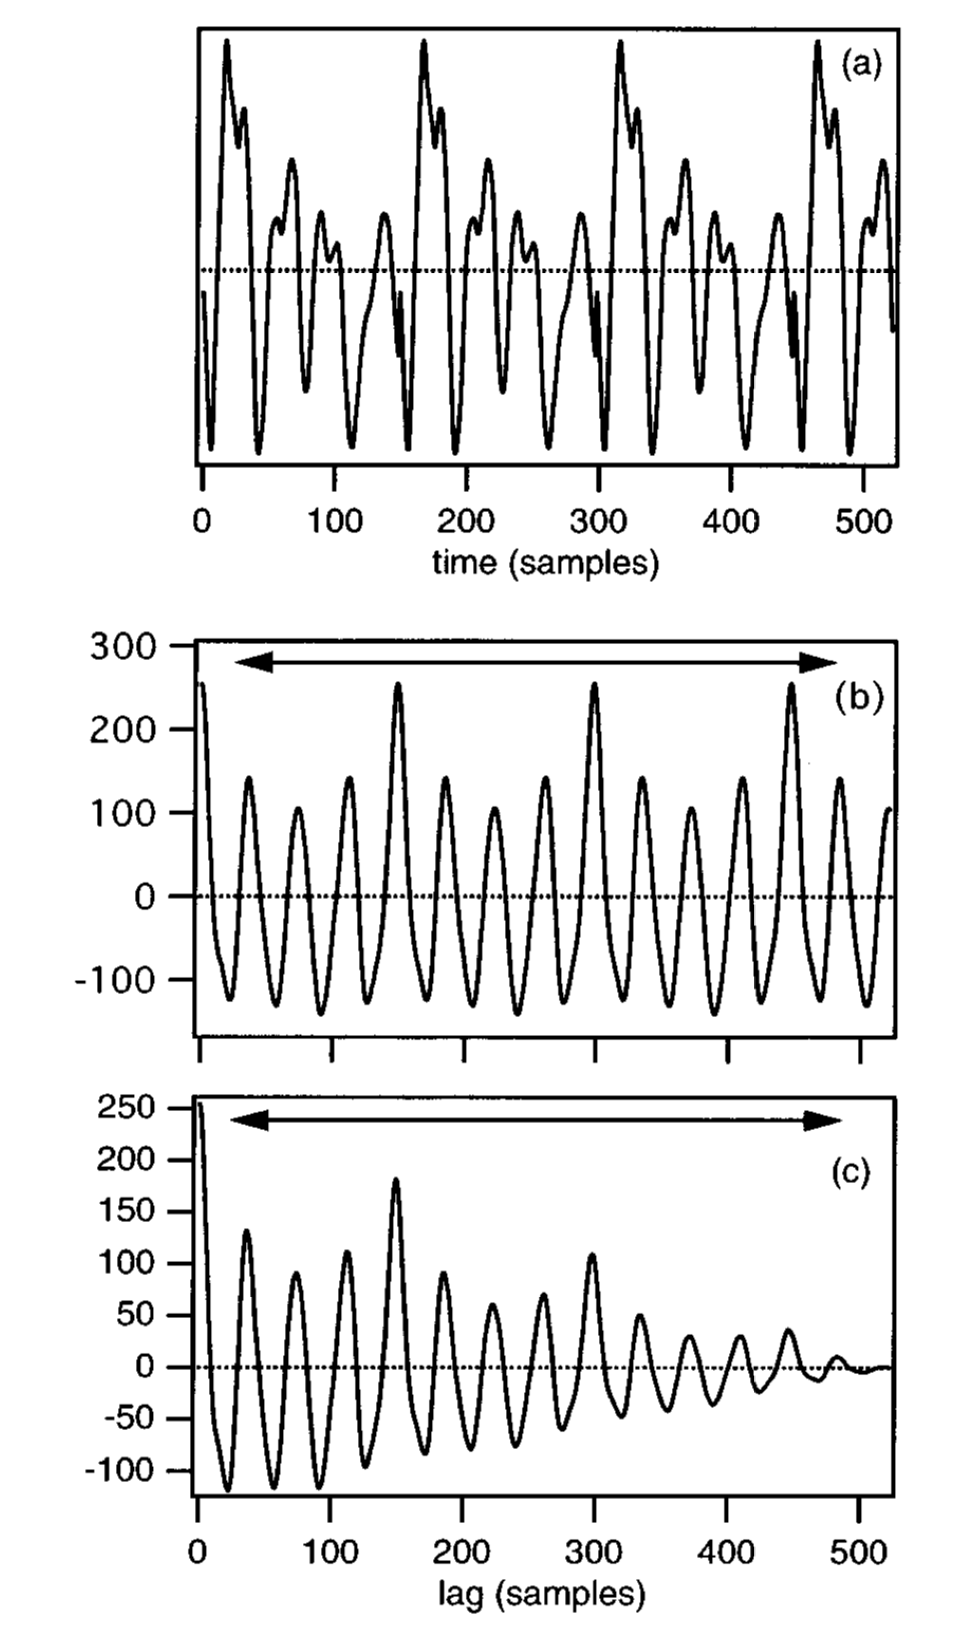
\includegraphics[width=\linewidth]{Image/Autocorreltation_3.png}
\end{minipage}
\begin{minipage}{0.5\textwidth}
\text{Autocorrelation Function}
\begin{equation}
r_t(\tau)=\sum_{j=t+1}^{t+W}x_{j}x_{j+\tau}
\end{equation}
\begin{equation}
r_{t}^{'}(\tau)=\sum_{j=t+1}^{t+W-\tau}x_{j}x_{j+\tau}
\end{equation}
The second largest peak location in samples gives $T_0$ and thus pitch is computed as:\\
\begin{equation}
F_0= F_s / T_0
\end{equation}
$F_s$: sampling frequency\\
$T_0$: pitch period in samples

\end{minipage}
\noindent

\end{frame}
%%%%%%%%%%
% Talk:
%  The analysis of autocorrelation is a mathematical tool for finding repeating patterns. It shows is the correlation(informally, similarity) of a signal with a delayed copy of itself as a function of lag \tau.

% This figure shows a voiced speech segment and its autocorrelation sequence. The pitch period information is more pronounced in the autocorrelation sequence comparing to the speech segment itself.

% The autocorrelation function(ACF) of a discrete signal x_t may be defined as shown is equation (1)
% \begin{equation}
% r_t(\tau)=\sum_{j=t+1}^{t+W}x_{j}x_{j+\tau}
% \end{equation}
% Where,
% rt(\tau): is the autocorrelation function of lag calculated at time index t
% W: integration window size

% Note: (Only positive lag values are shown in the figure. 
% Since autocorrelation sequence is symmetric with respect to zero lag, )

% It is common in signal processing to use a slightly different definition as shown in equation (2).
% \begin{equation}
% r_{t}^{'}(\tau)=\sum_{j=t+1}^{t+W-\tau}x_{j}x_{j+\tau}
% \end{equation}
% Here, the integration window size(W) shrinks with increasing values of \tau, with the result that the envelope of the function decreases as a function of lag as illustrated in Figure (c).

% In the second figure, the second largest peak is the autocorrelation sequence, represents To and can be picked up easily by a simple peak picking algorithm. (The largest is the signal itself).

%%% Optional
% Limitation:
% The main limitation of the autocorrelation method is that there may be peaks larger than the peak corresponding to the pitch period, due to the excitation of the vocal tract. As a result, there may be picking of wrong peaks and hence wrong estimation of pitch. 

% Solution: 
%  The approach to minimize such errors is to separate the vocal tract and excitation source related information in the speech signal,
% then use the source information for pitch estimation. 
    % -> Cepstrum Analysis, as the second method
%%%%%%%%%%

%------------------------
\begin{frame}
\frametitle{Cepstrum Pitch Determination}
\begin{figure}
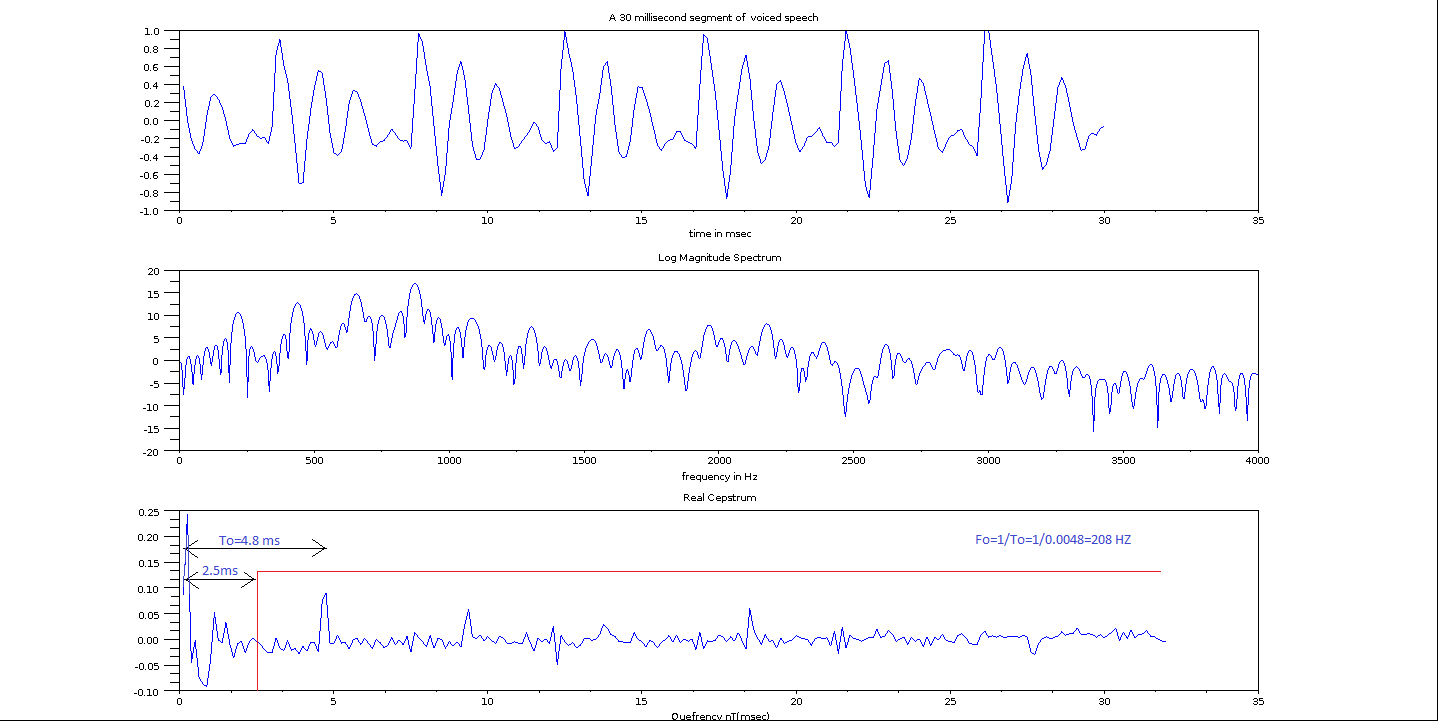
\includegraphics[width=0.8\linewidth]{Image/Fig6.png}
\end{figure}
The largest peak location gives $T_0$ and thus pitch is computed as:\\
\begin{equation}
F_0= 1 / T_0
\end{equation}
\hspace{10mm} $F_s$: sampling frequency \hspace{10mm} $T_0$: pitch period in time

% For Unvoiced data, the main distinction between cepstrum of voiced and unvoiced speech is:
% By comparing Fig 4 and Fig. 5 it may be observed that there is no prominent peak in case of ceptrum of unvoiced speech after the 13-15 initial cepstral values. 

%%%%%%%
% Talk
% Cepstrum
% The cepstrum of speech is defined as the inverse Fourier transform of the log magnitude spectrum.
% It projects (in log magnitude spectrum)
% slowly varying components -> low frequency region (of the cepstrum) -> vocal tract
% fast varying components ->high frequency region -> excitation source
% (The slowly varying components represent the envelope corresponds to the vocal tract and the fast varying components to the excitation source. As a result the vocal tract and excitation source components get represented naturally in the spectrum of speech.)

% As an example, this figure shows a 30 ms segment of voiced speech, 
% log magnitude spectrum 
% cepstrum

% Note that unvoiced speech will not have any prominent peak after 13-15 cepstral values. 

%  The initial few values in the cepstrum typically 13-15 cepstral values represent the vocal tract information. The large peak present after these initial values represent the excitation information. 
% In particular, the pitch period T0 starting from the zeroth value in number of samples. As a result the peaks that may be occurring in case of autocorrelation analysis get naturally eliminated cepstrum pitch determination. 
%%%%%%%
\end{frame}
%------------------------

\begin{frame}
\frametitle{Pitch estimation by SIFT method}
% Paper Link: https://www.researchgate.net/publication/3446031_The_SIFT_algorithm_for_fundamental_frequency_estimation

\textbf{Linear prediction (LP)\\}
% https://link.springer.com/content/pdf/bbm%3A978-1-4614-5143-3%2F1.pdf

%%%%%%%
% The Single Inverse Filter Tracking(SIFT) method Based on the linear prediction (LP) analysis of speech. That is, it approximated a speech sample as a linear combination of past samples. (It in turn employs the autocorrelation method)
%%%%%%
- A speech sample can be approximated as a linear combination of past samples. \\
- Obtain a unique set of predictor coefficients by minimizing the sum of the squared differences between the actual speech samples and the linearly predicted ones over a finite interval.\\
- Decomposes the speech into two highly independent components:\\
\hspace{10mm} 1. Vocal tract parameters (LP coefficients)\\
\hspace{10mm} 2. Glottal excitation (LP residual).\\
%%%%%%
% Then SIFT performs autocorrelation of the LP residual than speech directly.
%%%%%%
% It is assumed that speech is produced by exciting a linear time-varying filter (the vocal tract) by random noise for unvoiced speech segments, or a train of pulses for voiced speech.
- The autocorrelation of LP residual will therefore have unambiguous peaks representing the pitch period 'T0' information.
%%%%%%
\end{frame}

%------------------------

\begin{frame}
\frametitle{Pitch estimation by SIFT method}
\begin{figure}
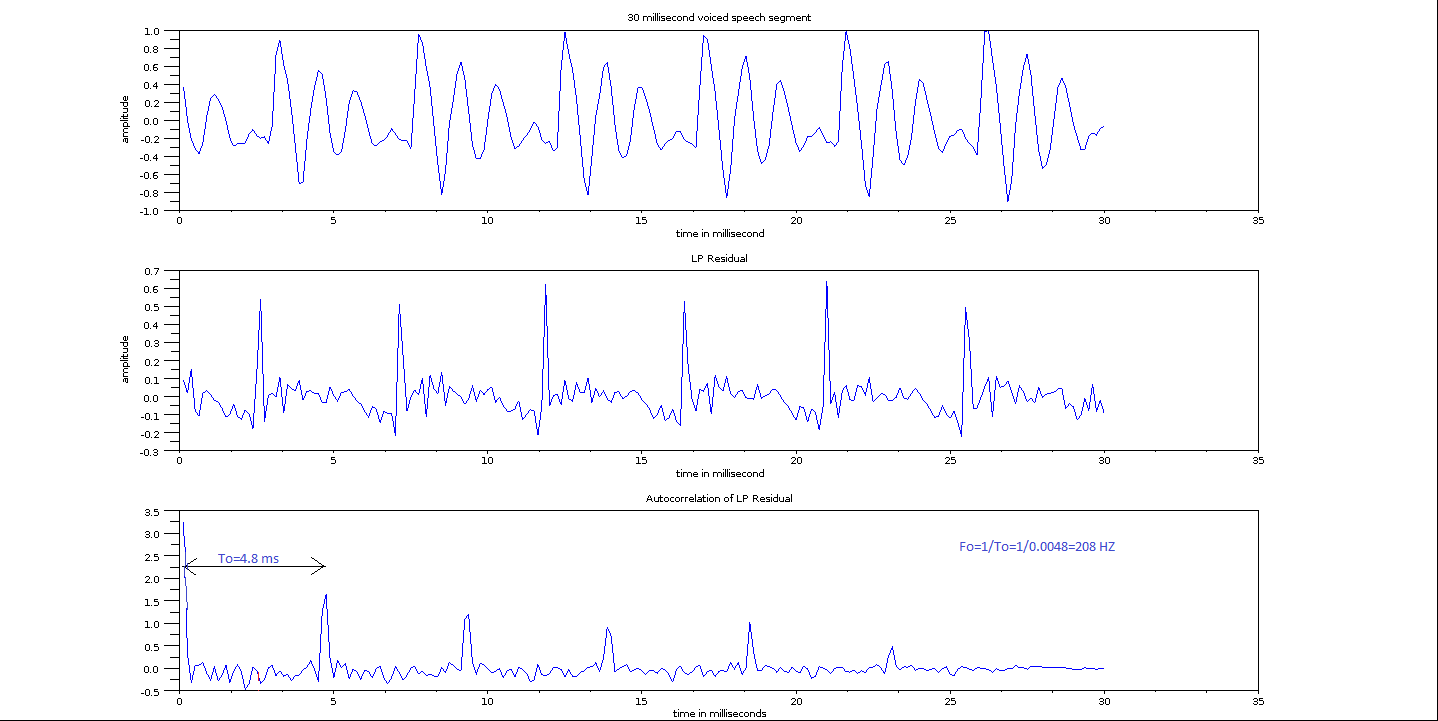
\includegraphics[width=0.8\linewidth]{Image/Fig9.png}
\end{figure}
% Figure above shows a 30 msec segment of voiced speech, its LP residual and the autocorrelation of the LP residual. \\
% As can be observed, there is a prominent peak at the pitch period 'T0' and there are no other peaks that interfere with its peak. This is the merit of SIFT over autocorrelation of speech.
% There is no prominent peak in the autocorrelation of LP residual for unvoiced signals
A single peak picking can be employed for the estimation of pitch period $T_0$ as illustrated in the figure. 
Pitch is computed as:\\
\begin{equation}
F_0 = 1 / T_0
\end{equation}
\hspace{10mm} $F_s$: sampling frequency \hspace{10mm} $T_0$: pitch period in time
\end{frame}

%%%%% Summary
% Cepstral and the SIFT method sequences have less ambiguity compared to autocorrelation of speech. Hence either cepstrum or SIFT method is equally preferable for the estimation of pitch. In case of speech coding, the mostly used are in LP analysis and hence SIFT method is preferred over Cepstrum pitch estimation. Alternatively, in tasks like speaker recognition, since cepstral analysis is used for the feature extraction tasks, cepstrum pitch estimation may be employed.

%------------------------------------------------
\section{Motivation} 
%------------------------------------------------
\subsection{pYIN Pitch Estimation}
%------------------------
\begin{frame}
\frametitle{Baseline: YIN and pYIN}
\begin{figure}
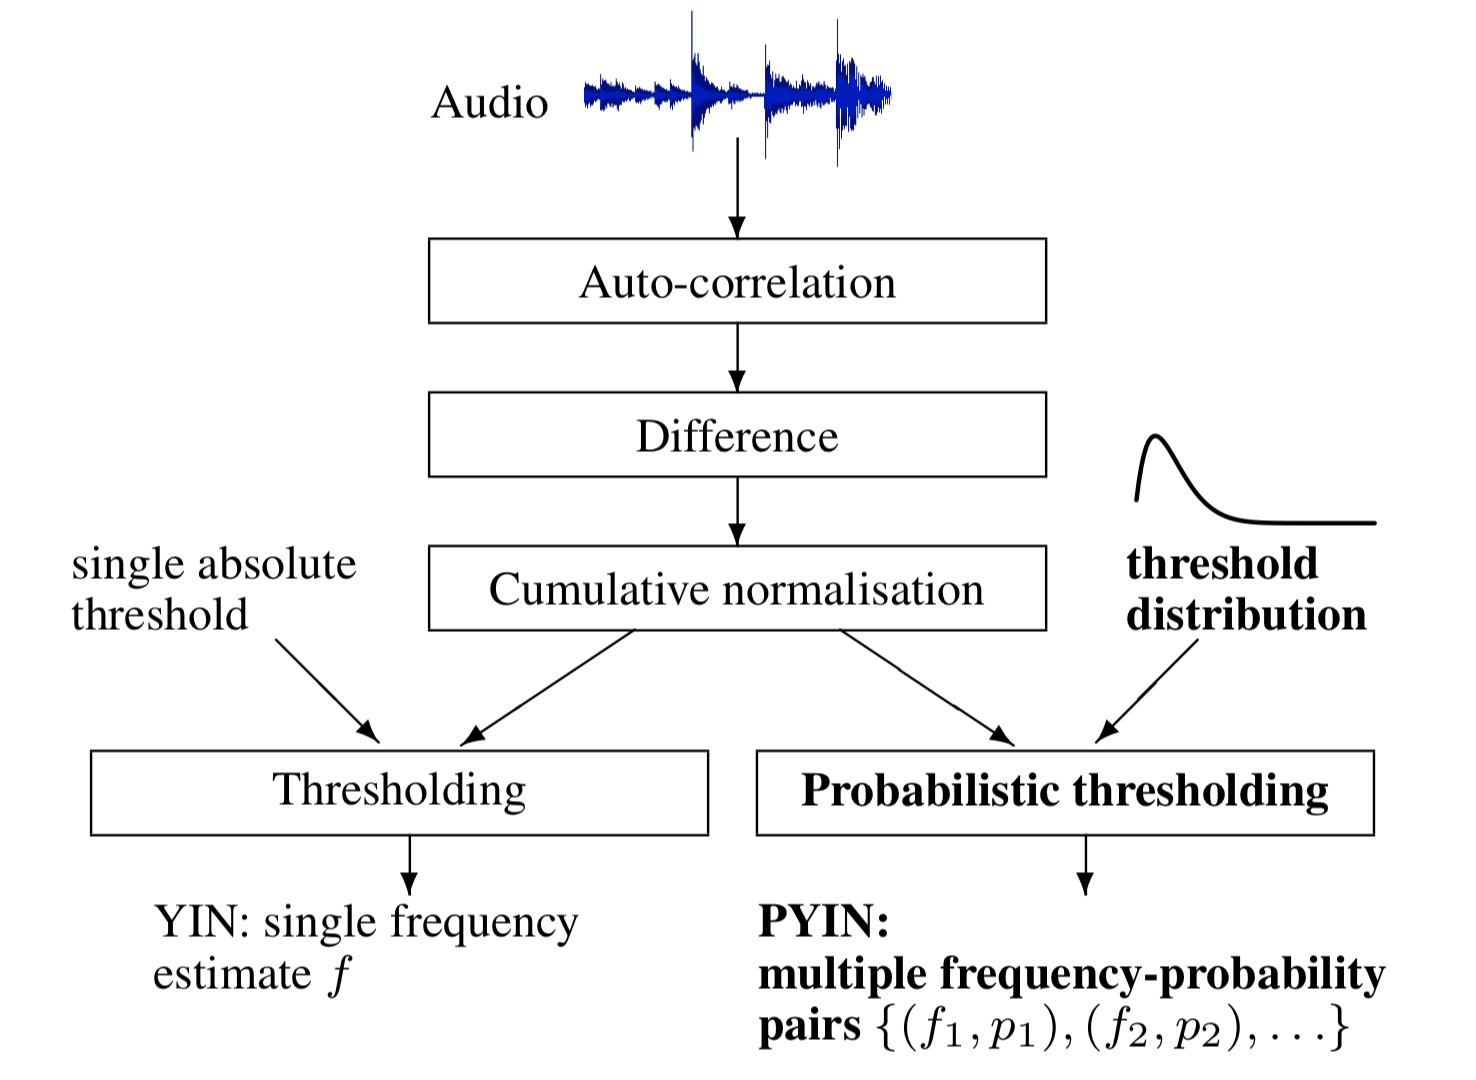
\includegraphics[width=0.8\linewidth]{Image/YIN_and_pYIN.png}
\end{figure}
\end{frame}

% %------------------------
% \begin{frame}
% \frametitle{Baseline: YIN and pYIN - Error Mechanisms }
% \textbf{Difference Function}
% \begin{equation}
%     d_t(\tau) = \sum_{j=1}^{W}(x_j - x_{j+\tau})^2
% \end{equation}
% Searching for the values of $\tau$ for which the function is zero to obtain $T_0$. Expand the square sum and express in terms of the ACF:
% \begin{equation}
%     d_t(\tau) = r_t(0) + r_{t+\tau}(0) - 2r_t(\tau)
% \end{equation}
% %%%%%%
% % Note that the 2nd and 3rd terms both varies w.r.t. \tau.
% % Our goal is to find a \tau that drags the difference function as close to 0 as possible. This is been shown to largely reduce the error rate of pitch estimation.
% %%%%%%

% \textbf{Cumulative Normalization}
% \begin{equation}
%     d_t^{'}(\tau) = \begin{cases} 
%                     1, \hspace{10mm} if\tau = 0,\\
%                     \frac{d_t(\tau)}{[(1/\tau) \sum_{j=1}^{\tau}d_t(j)]}, \hspace{5mm} otherwise.
%                     \end{cases}
% \end{equation}

% %%%%%%
% % This new function is obtained by dividing each value of the old by its average over shorter-lag values. This is used to replace the difference function to avoid some defects such as error introduced by zero-lag values. This is followed by other error-reduction step.

% % The YIN method then sets an absolute threshold and choose the smallest value of \tau that gives a minimum of d'(\tau) deeper than that threshold.
% % While the variant of YIN, pYIN then use these probabilities as observations in a Hidden Markov Model, to produce an improved pitch track.
% %%%%%%
% \end{frame}

%------------------------------------------------
\subsection{SWIPE Pitch Estimation}
%------------------------
\begin{frame}
\frametitle{Baseline: SWIPE Pitch Estimation}
Sawtooth Waveform Inspired Pitch Estimator(SWIPE)
\begin{figure}
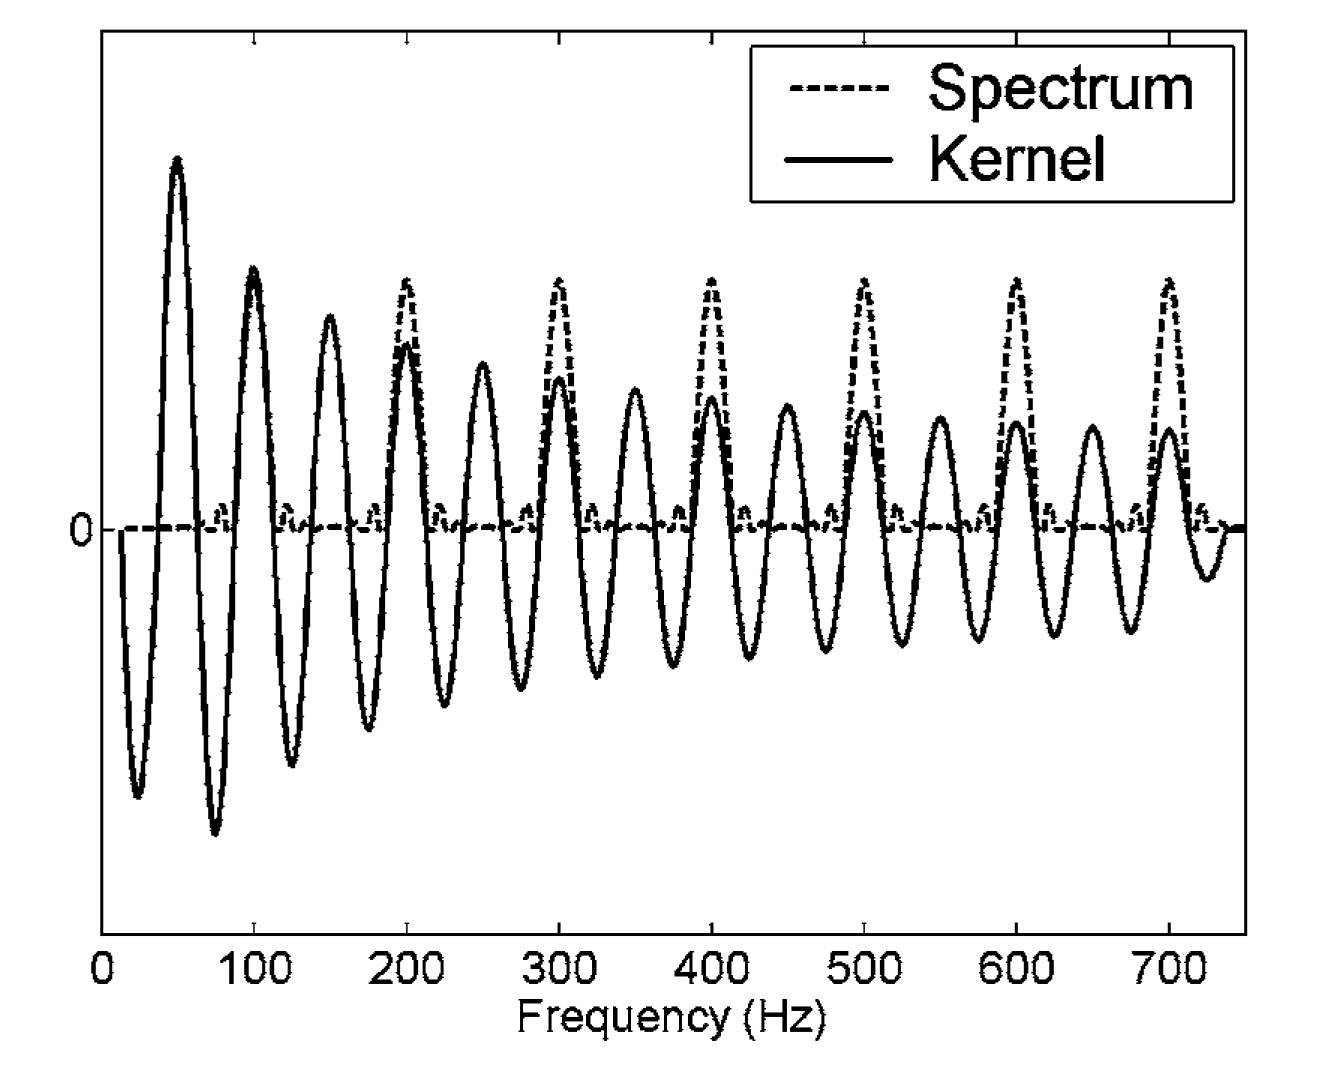
\includegraphics[width=0.6\linewidth]{Image/SWIPE_kernel.png}
\end{figure}

%%%%%
% Another state-of-the-art result is obtained by another model called SWIPE, a Saw-tooth Waveform Inspired Pitch Estimator. It is also used as the baseline for our paper. This estimator uses different approach from previous mentioned ones, it estimates the pitch as the fundamental frequency of the kernel waveform, whose spectrum best matches the spectrum of the input signal. The kernel functions can be either parabola, cosine, or Gaussian kernels, there is no significant difference in terms of performance between them. (Note that their approach determine pitch but not fundamental frequency(F0))

% The harmonics of pitch plays an important role in this approach as well, which is can be a source of error even with some methods to eliminate the defects. 

% (This approach utilizes the measurement of the global Average Peak-to-Valley Distance (APVD) at harmonic locations as well.)
%%%%%

\end{frame}

%------------------------------------------------
\subsection{Shortcomings of existing methods and Motivation}
\begin{frame}
\frametitle{Shortcomings of existing methods and Motivation}
\begin{itemize}
\item The development of well-performed systems solely depends on devising a robust \textbf{candidate-generating function}(i.e. heuristics) % like the complex estimation of the kernel function of SWIPE.
and/or \textbf{sophisticated post-processing steps}. % Like the various error-reduction algorithms used in pYIN
\item \textbf{None} of the model \textbf{directly learn from data}, except for manual hyper-parameter tuning. 
\item In \textbf{other problems} in music information retrieval, e.g. chord ID, beat detection, \textbf{data-driven methods have been shown consistently out-perform heuristic approaches}.
\item Current methods still produce noisy results for uncommon instruments and highly fluctuated pitch curves. 
\end{itemize}

\end{frame}
%------------------------------------------------
\section{Method}
%------------------------------------------------
\subsection{CREPE - Architecture}
\begin{frame}
\frametitle{CREPE - Architecture}
\begin{figure}
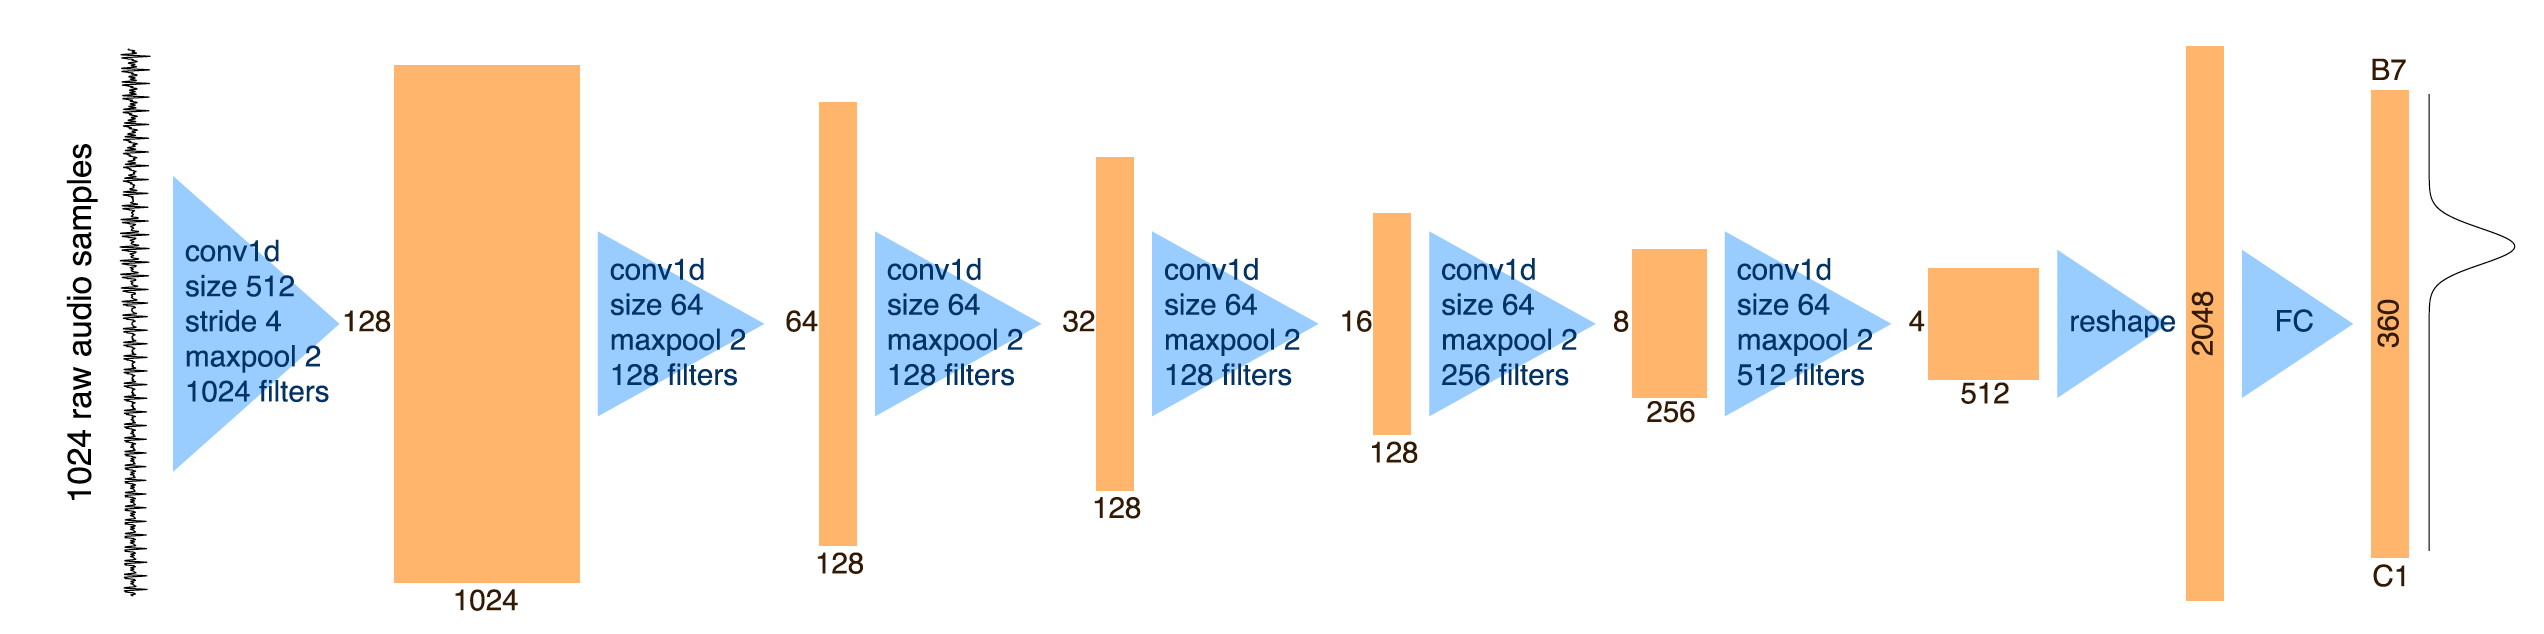
\includegraphics[width=\linewidth]{Image/CREPE_CNN.png}
\end{figure}
\begin{itemize}
\item Input: 1024 samples excerpt from time-domain audio signal, 16kHz sampling rate.
\item 6 convolutional layers, resulting in 2048 latent representation
\item Sigmoid activation, deterministic
\item 360-dim output vector where each frequency bin covers 20 \textbf{cents}.
\end{itemize}
\end{frame}

%--------------------
\begin{frame}
\frametitle{CREPE - Output Interpretation}
% Each of the 360 nodes in the output layer corresponds to a specific pitch value, defined in \textbf{cents}.
\textbf{Cent}: A unit representing musical intervals relative to a reference pitch $f_{ref}$ in $Hz$, defined as a function of frequency f in Hz:
\begin{equation}
    c(f) = 1200 \times log_2 \frac{f}{f_{ref}} 
\end{equation}
Where $f_{ref} = 10Hz$ is used throughout the experiment. The 360 pitch values are denoted $c_1, c_2, ..., c_{360}$, covers \textbf{6 octaves} from \textbf{C1} to \textbf{B7}. \\
Resulting pitch estimate $\hat{c}$ is the weighted average of the associated $c_i$.
\begin{equation}
    \hat{c}(f) = \frac{\sum_{i=1}^{360}\hat{y_i}c_i}{\sum_{i=1}^{360}\hat{y_i}}
\end{equation}
and obtain the estimated frequency:
\begin{equation}
    \hat{f} = f_{ref}\times 2^{\hat{c}/1200}
\end{equation}
\end{frame}


%------------------------------------------------
\subsection{CREPE - Datasets}
\begin{frame}
\frametitle{CREPE - Datasets}
\textbf{RWC-syth}
\begin{itemize}
\item \textbf{6.16 hours} of audio synthesized from the RWC Music Database.
\item Have perfect control over the $F0$ of the resulting signal.
\item Synthesized using a fixed sum of a small number of sinusoidal, highly homogeneous in timbre and represents an \textbf{over-simplified scenario.}
\end{itemize}
\textbf{MDB-stem-synth}
\begin{itemize}
\item 230 tracks with 25 instruments, totaling 15.56 hours of audio.
\item Monophonic stems taken from MedleyDB and re-synthesized, with a \textbf{perfect f0 annotation} that \textbf{maintains the timbre and dynamics} of the original track.
\item Representing a \textbf{real-world scenario}.
\end{itemize}
\end{frame}

%--------------------
\begin{frame}
\frametitle{CREPE - Target Output and Training}
\textbf{Target Output}\\
360-dimensional vector(same as model's output). Frequency bin with the ground truth frequency is given a magnitude of 1 and then Gaussian blurred.
\begin{equation}
    y_i = exp(-\frac{(c_i-c_{true})^2}{2\times25^2})
\end{equation}
%%%%%
% So that the energy surrounding a ground truth frequency decays with a standard deviation of 25 cents. 
% Therefore, the input pitch is close to the associated frequency bins with high activation.
%%%%%

\textbf{Cross entropy loss} between predicted vector $\hat{y}$ and target vector $y$\\
\begin{equation}
    L(y, \hat{y}) = \sum_{i=1}^{360}(-y_i log\hat{y_i}-(1-y_i) log(1-\hat{y_i}))
\end{equation}
\begin{itemize}
\item Optimized by ADAM optimizer with learning rate 0.0002.\\
\item Trained for 32 epochs with 500 batches and batch size 32.\\
\item Each convolutional layer is followed with a drop out layer with drop-out rate 0.25.
\end{itemize}
\end{frame}

%------------------------------------------------
\section{Experiment and Results}
%------------------------------------------------

\subsection{Experiment and Evaluation Criteria}
\begin{frame}
\frametitle{Experiment and Evaluation Criteria}
\textbf{Methodology}\\
\hspace{5mm}5-fold cross-validation, 60/20/20 train, validation and test split.\\

\textbf{Evaluation}\\
\hspace{5mm}Raw Pitch Accuracy(RPA) and Raw Chorma Accuracy(RCA) within 50 cent(a quarter-tone) threshold of the ground truth.

\textbf{Added Noise - Audio Degradation Toolbox(ADT)}\\
\hspace{5mm}4 Noise sources: pub, while, pink, brown\\
\hspace{5mm}Use different Signal-to-Noise Ratios(SNR): $\infinity, 40, 30, 20, 10, 5, 0dB$
% pub noise: an actual recording of the sound in a crowded pub
% white noise: a random signal with a constant power spectral density over all frequencies. 
% pink and brown noise: have the highest power spectral density in low frequencies, and the densities fall off at 10 dB and 20 dB per decade respectively.

\end{frame}
%------------------------------------------------
\subsection{Results}
%-----------------------
\begin{frame}
\frametitle{Results - Pitch Accuracy with 50 cents(standard) threshold}
\textit{Table 1. Average raw pitch/chroma accuracies and their standard deviations, tested with the 50 cents threshold}
\begin{figure}
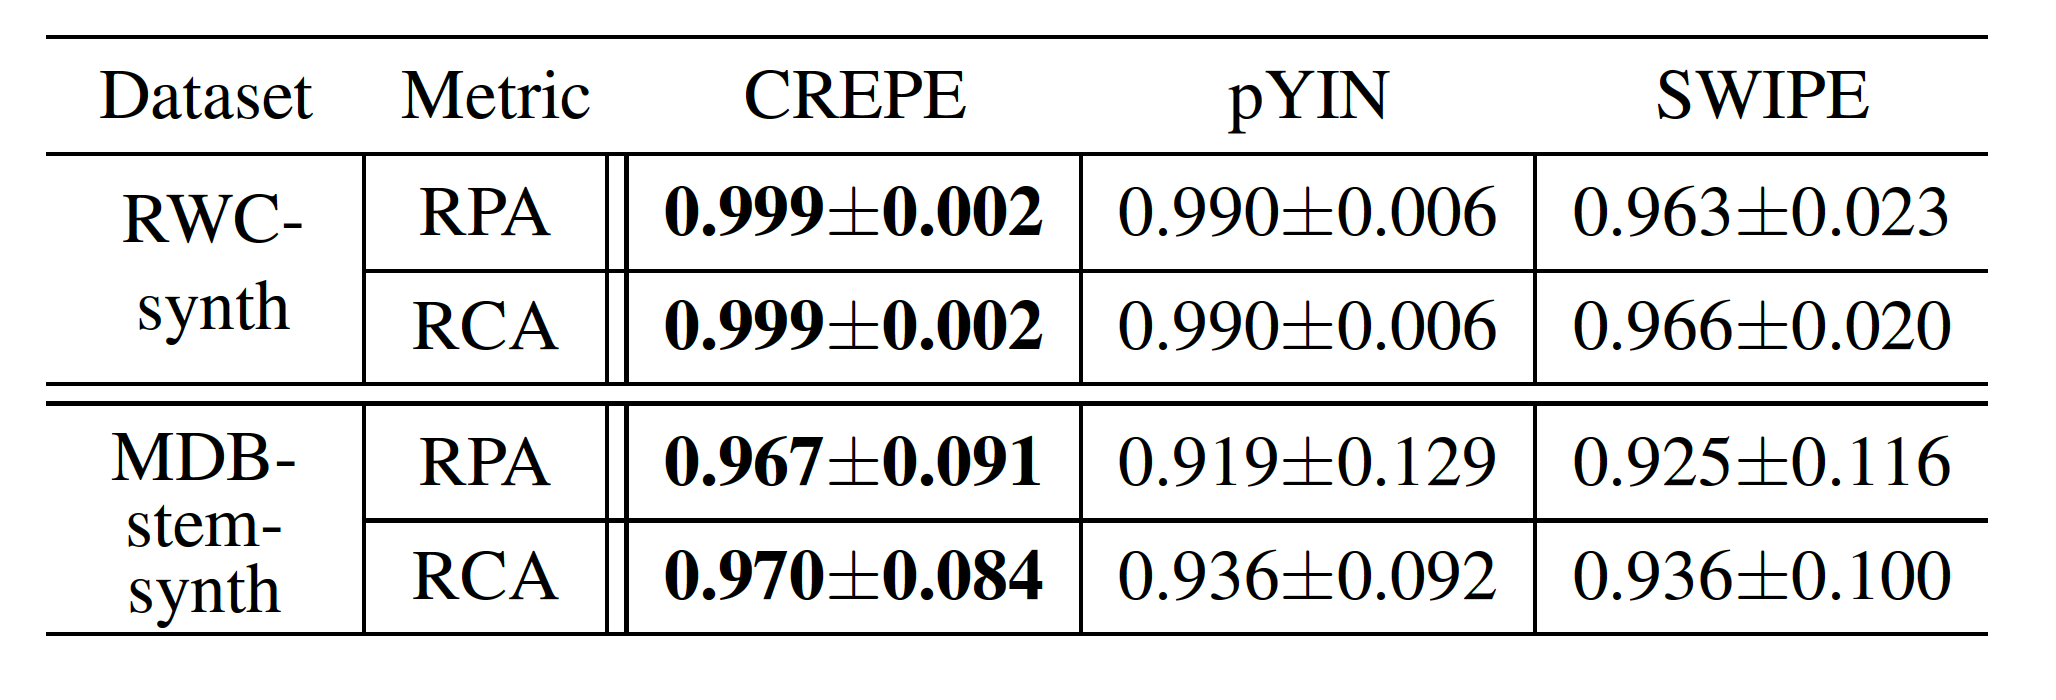
\includegraphics[width=0.9\linewidth]{Image/Table_1.png}
\end{figure}
%%%%%
% RWC-synth: highly homogeneous timbre -> higher accuracy
%%%%%
\end{frame}
%---------------------
\begin{frame}
\frametitle{Results - Pitch Accuracy with different evaluation thresholds}
\textit{Table 2: Average raw pitch accuracies and their standard deviations, with different evaluation thresholds.}
\begin{figure}
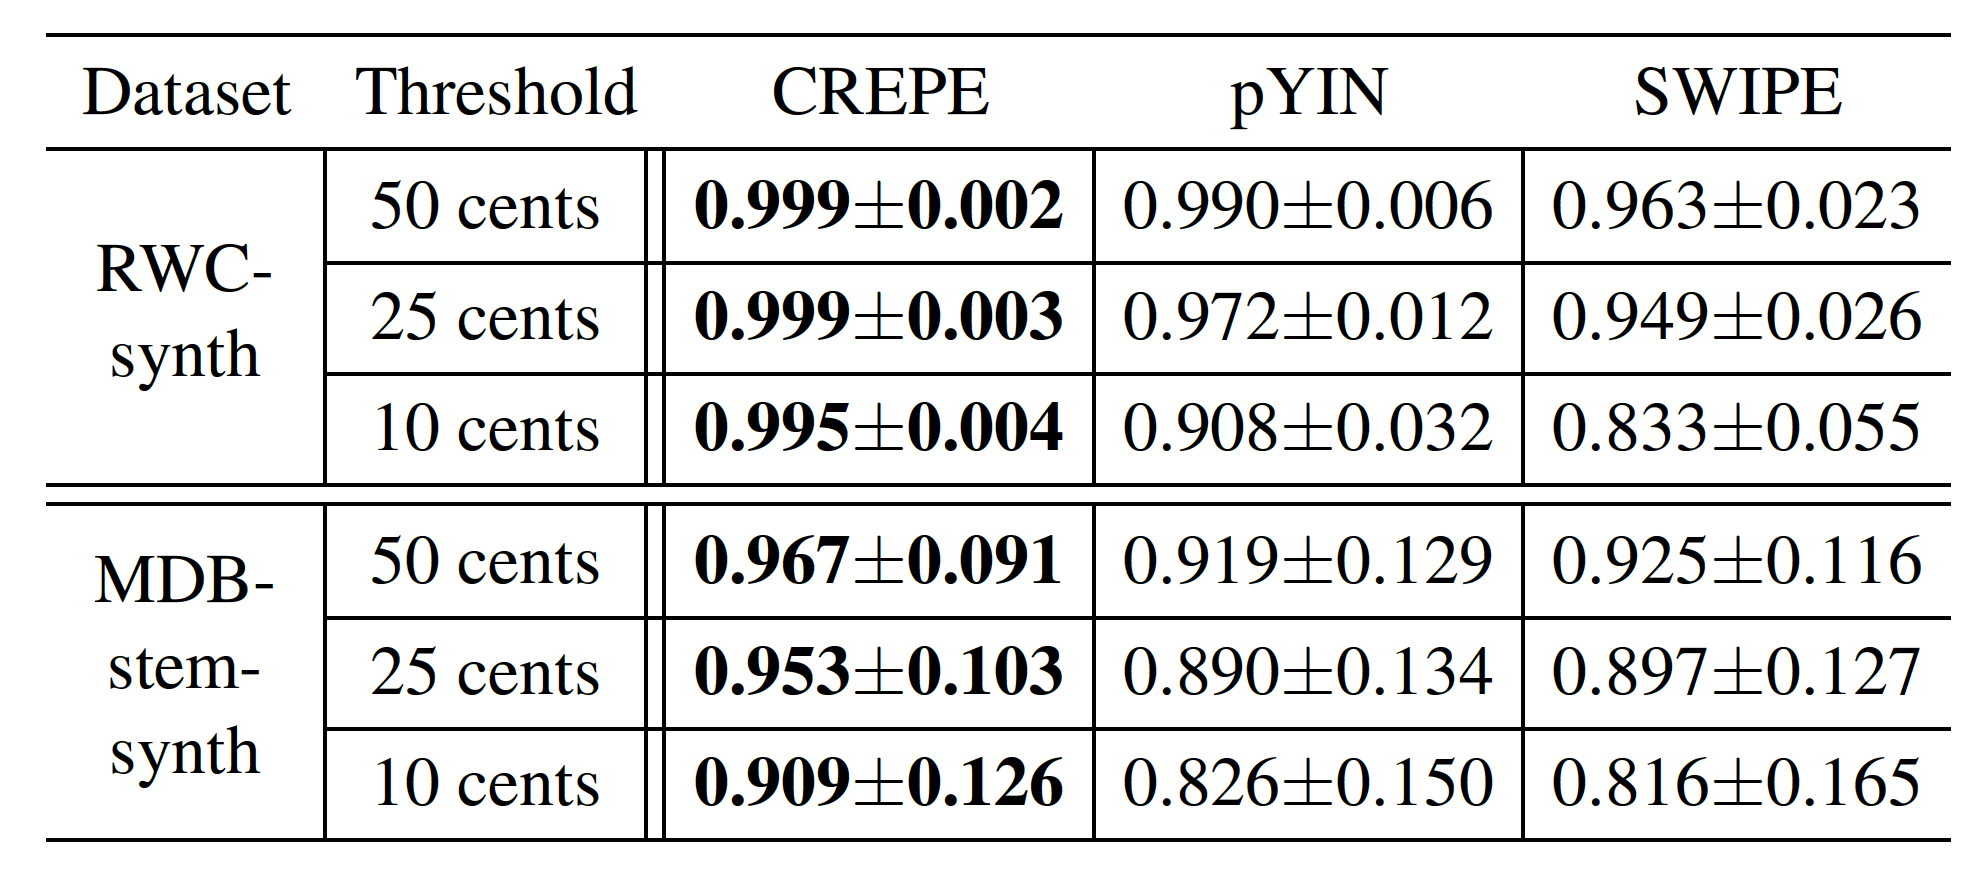
\includegraphics[width=0.85\linewidth]{Image/Table_2.png}
\end{figure}
This suggests that CREPE is especially preferable when even minor deviations from the true pitch should be avoided as best as possible.
%%%%%
% As the threshold is decreased, the difference in performance becomes more accentuated. 
%%%%%
\end{frame}
%--------------------
\begin{frame}
\frametitle{Results - Niose Robustness}
\textit{Pitch tracking performance when additive noise signals. \\
The error bars are centered at the average raw pitch accuracies and span the first standard deviations. \\
With brown noise being a notable exception, CREPE shows the highest noise robustness in general.} 
\begin{figure}
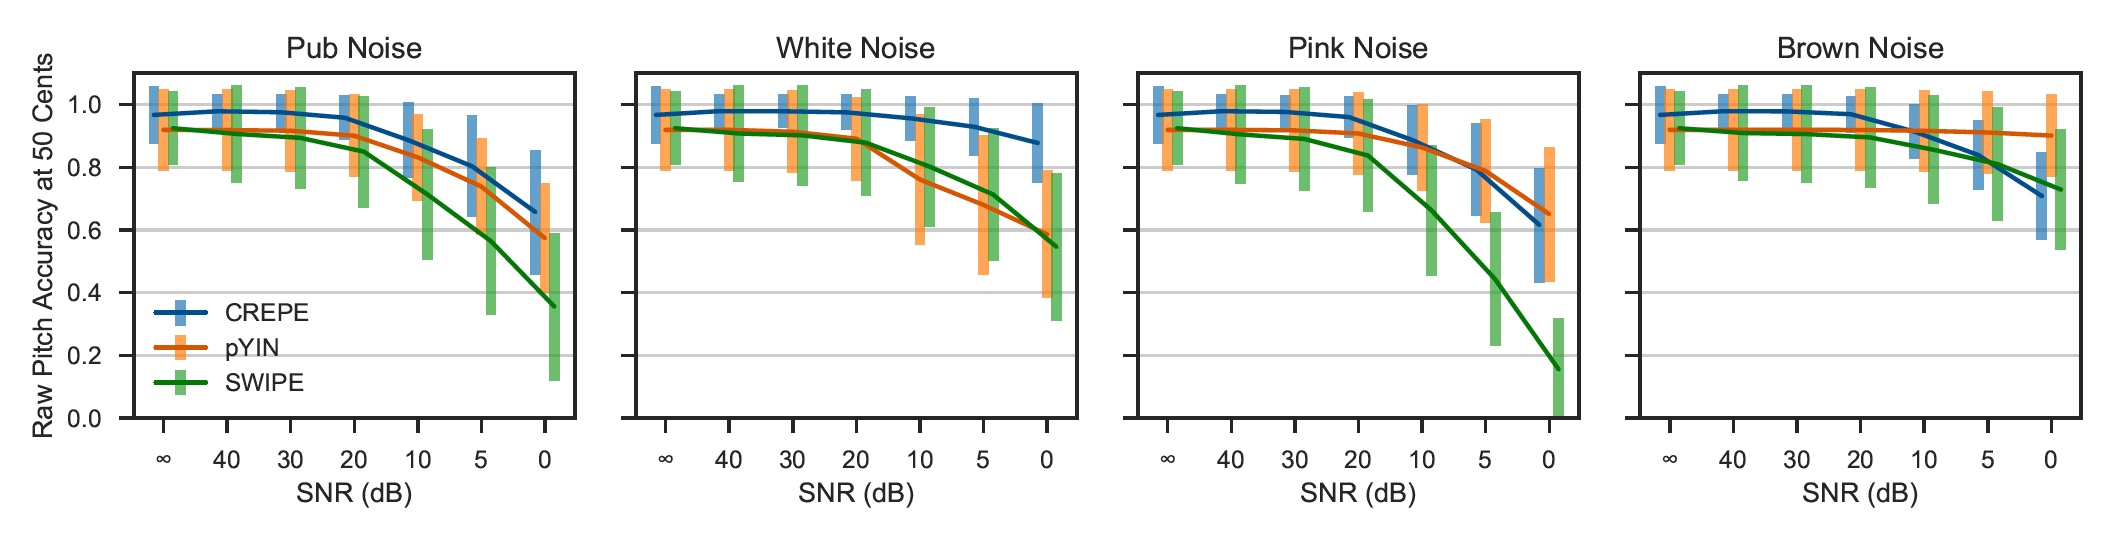
\includegraphics[width=\linewidth]{Image/Robustness.png}
\end{figure}
\end{frame}
%--------------------
\begin{frame}
\frametitle{Results - Performance by Instrument}
\textit{RPA of CREPE’s predictions on each of the 230 tracks in MDB-stem-synth with respect to the instrument, sorted by the average frequency.} 
\begin{figure}
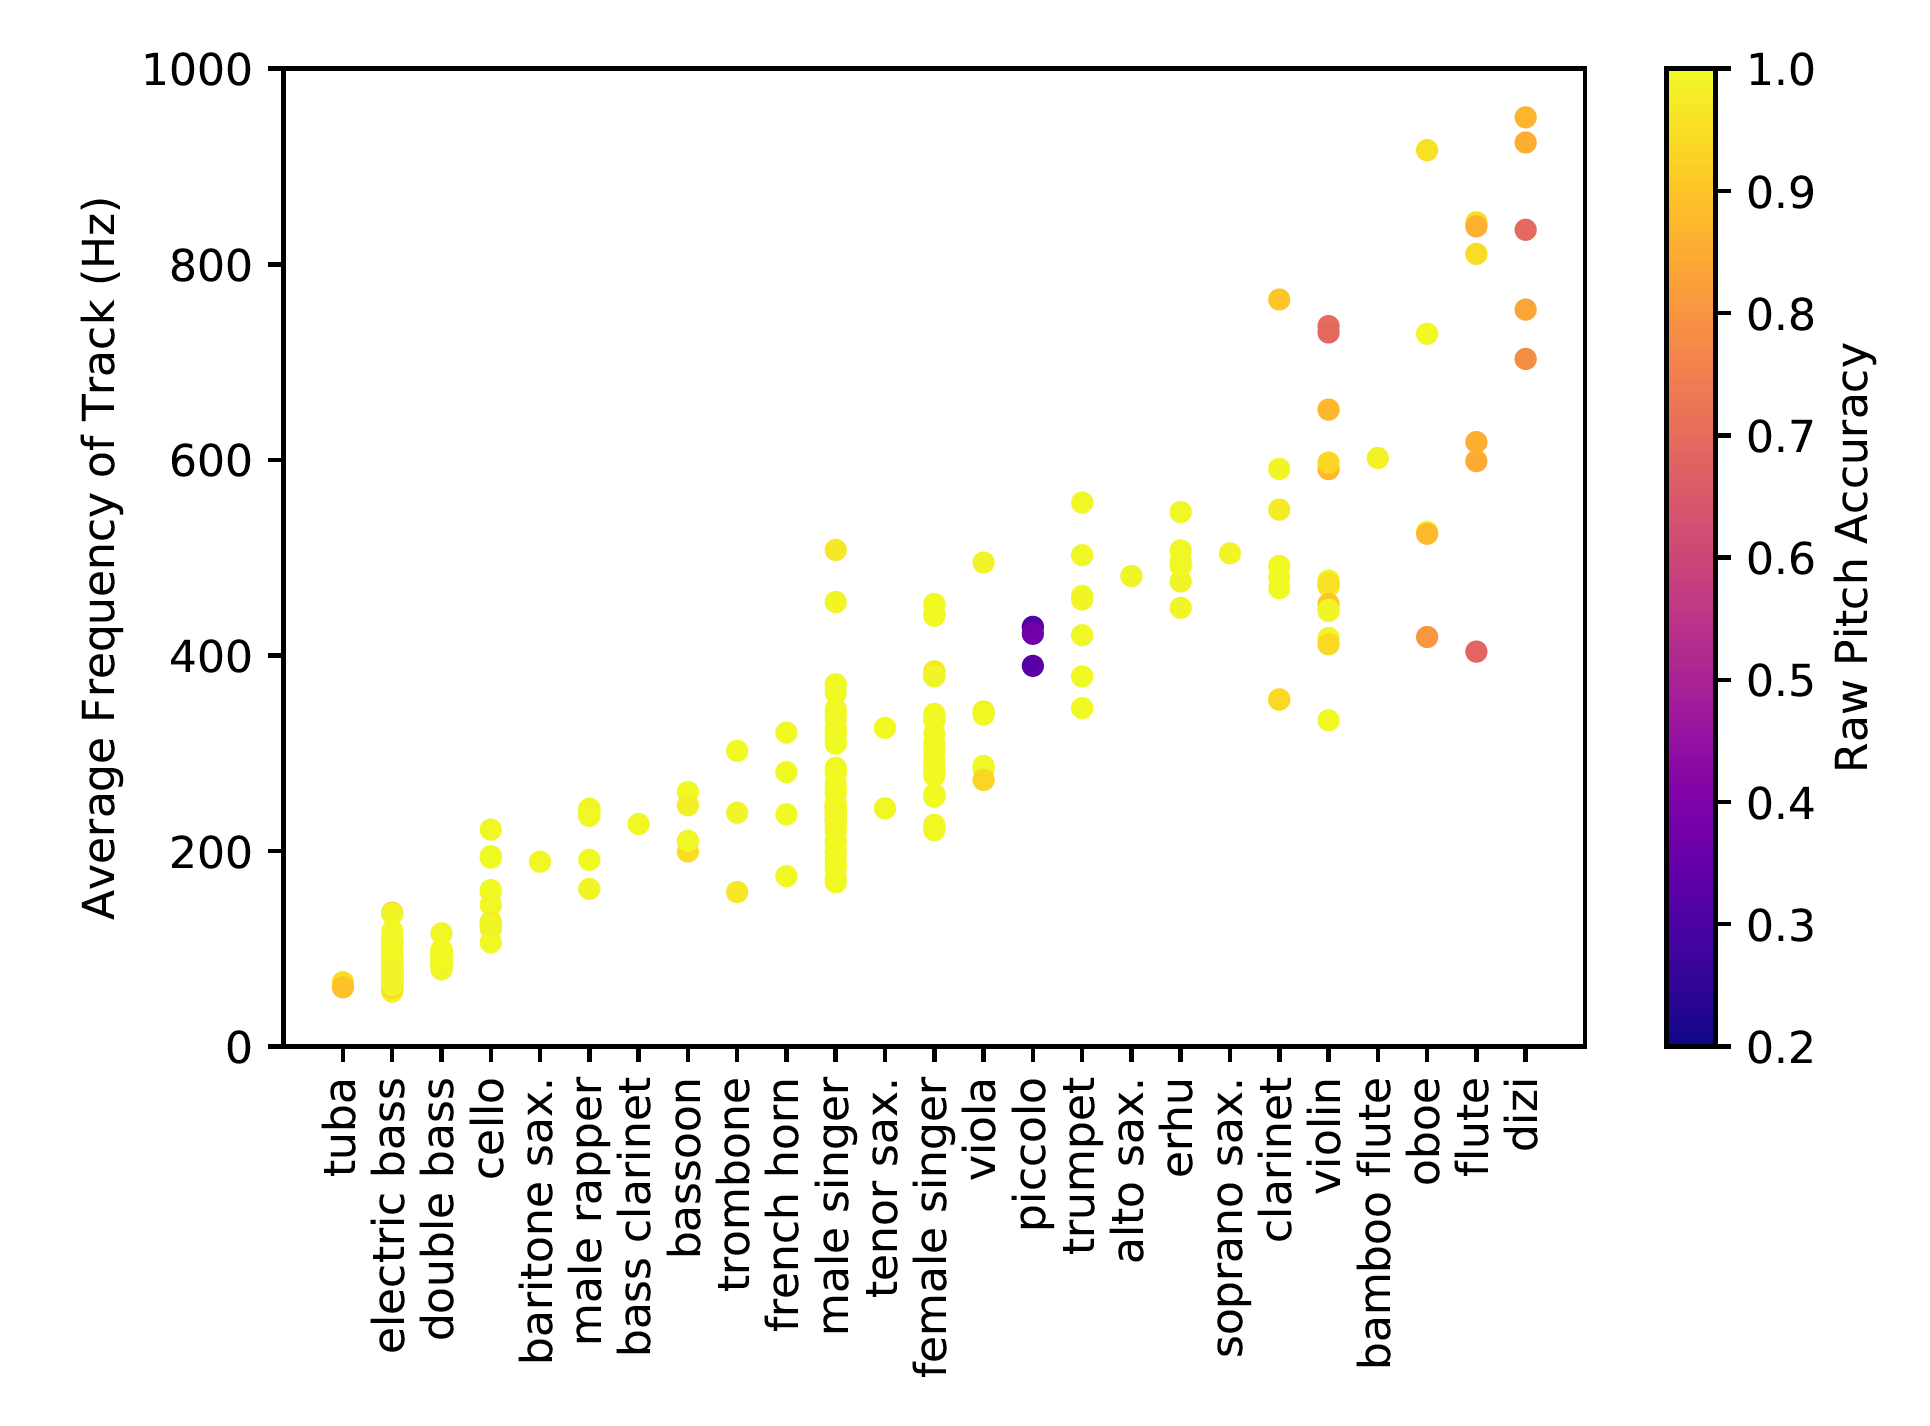
\includegraphics[width=0.83\linewidth]{Image/Instruments.png}
\end{figure}
%%%%%%
% Exceptions:
% Dizi: Failed to generate previously unseen timbre
% Poccolo: wrong label in the dataset
% Others like bamboo flute and bass clarinet: have similar timbre so high accuracy
%%%%%%
\end{frame}

%------------------------------------------------
\section{Discussion and Conclusion}
%------------------------------------------------
\subsection{Discussion and Conclusion}
%---------------------
\begin{frame}
\frametitle{Conclusion}
\textbf{Contribution of this model}\\
\begin{enumerate}
    \item State-of-the-art performance on both datasets with homogeneous and heterogeneous timbre.
    \item Highly accurate even at strict evaluation threshold.
    \item More robust to added noise.
    \item Innovative data-driven pitch tracking algorithm.
\end{enumerate}

\textbf{Future Work}\\
\begin{enumerate}
    \item Model should be invariant to all transformations that do not effect pitch. Use data augmentation to generate transformed and degraded signal and make the model to learn the invariance.  %Currently the model have pooling layer to reduce translation invariance
    \item Robustness can be improve by applying pitch-shift to cover a wider pitch range.
    \item Enforcing temporal smoothness to improve the performance, by using CRNN.
\end{enumerate}
\end{frame}
%--------------------

\begin{frame}
\Huge{\centerline{Q \& A}}
\end{frame}

%----------------------------------------------------------------------------------------

\end{document}